\documentclass[11pt,a4paper]{article}
\usepackage[utf8]{inputenc}
\usepackage[T1]{fontenc}
\usepackage[brazil]{babel}
\usepackage{lmodern}
\usepackage[margin=2cm]{geometry}
\usepackage{amsmath,amssymb}
\usepackage{booktabs}
\usepackage{graphicx}
\usepackage{hyperref}
\usepackage{xcolor}
\usepackage{titlesec}
\usepackage{tabularx}
\usepackage{enumitem}
\usepackage{float}
\usepackage{array}
\renewcommand{\tabularxcolumn}[1]{>{\raggedright\arraybackslash}p{#1}}

\hypersetup{
    colorlinks=true,
    linkcolor=blue!70!black,
    citecolor=blue!70!black,
    urlcolor=blue!70!black
}

\titleformat{\section}{\large\bfseries}{\thesection.}{0.5em}{}
\titleformat{\subsection}{\normalsize\bfseries}{\thesubsection.}{0.5em}{}
\titlespacing*{\section}{0pt}{1.2ex plus 0.5ex minus .2ex}{0.6ex}
\titlespacing*{\subsection}{0pt}{1.0ex plus 0.4ex minus .2ex}{0.4ex}

\setlength{\parskip}{0.45em}
\setlength{\parindent}{0pt}
\setlist{itemsep=0.15em,topsep=0.3em}

\begin{document}

\begin{center}
    {\LARGE \textbf{Relatório de Status do TCC}} \\[0.35em]
    {\large Avaliação das Explicações SHAP em Redes Neurais Profundas para Classificação de Arritmias Cardíacas em ECG} \\[0.3em]
    \textbf{Aluno:} Arthur Santos de Oliveira (RA: 156297) \\[0.2em]
    \textbf{Orientador:} Prof.\ Dr.\ Luis Augusto Martins Pereira \\[0.2em]
    \textbf{Data:} 20/10/2026 \\[0.2em]
    \textbf{Repositório:} \url{https://github.com/Arthur-so/shap-ecg-arrhythmia}
\end{center}
\vspace{-0.5em}
\hrule
\vspace{0.8em}

\section{Resumo}

\begin{itemize}
    \item O classificador está no nível do artigo base: F1-macro de \textbf{0,819} no teste, contra 0,813 de Zhang et al. (2021).
    \item Desde o último relatório (14/10), a \textbf{Faithfulness Estimate} foi revisada, \textbf{reimplementada} e calculada. Já são três métricas de qualidade das explicações calculadas e documentadas: \textbf{Consistency}, \textbf{Faithfulness Correlation} e \textbf{Faithfulness Estimate}. As três foram reimplementadas a partir dos artigos originais, porque as versões do Quantus não eram adequadas ao ECG.
    \item As três métricas, lidas em conjunto, mostram que as explicações SHAP refletem o modelo de forma moderada e que a qualidade delas \textbf{acompanha o F1 só em parte}: parece depender também do tipo de classe (seção~5).
    \item A \textbf{complexidade}, terceiro critério do artigo da Faithfulness Correlation, foi analisada; propõe-se incluí-la como métrica complementar.
    \item A \textbf{Sufficiency} segue retirada, e as demais métricas continuam em revisão.
\end{itemize}

\section{Modelo avaliado}

ResNet34 1D treinada no CPSC2018 (9 classes), com o protocolo de Zhang et al. (2021), perda BCE simples e limiar de decisão por classe. As explicações GradientSHAP foram geradas para as \textbf{622 predições corretas} do conjunto de teste. Todas as métricas abaixo usam o mesmo modelo e os mesmos mapas.

\section{Métricas: o que foi decidido e por quê}

\subsection{Base comum: regiões do batimento}
Um mapa SHAP tem 180\,000 valores (12 derivações × 15\,000 instantes), e um ponto isolado do ECG não tem significado clínico. Por isso, as métricas reimplementadas usam os mesmos \textbf{atributos}: cada batimento é dividido, a partir do pico R, em três partes (pré-QRS, QRS e ST-T), em cada uma das 12 derivações, o que dá \textbf{36 regiões} por ECG (Figura~\ref{fig:regioes}). A importância de uma região é a soma do mapa SHAP nela.

\begin{figure}[H]
\centering
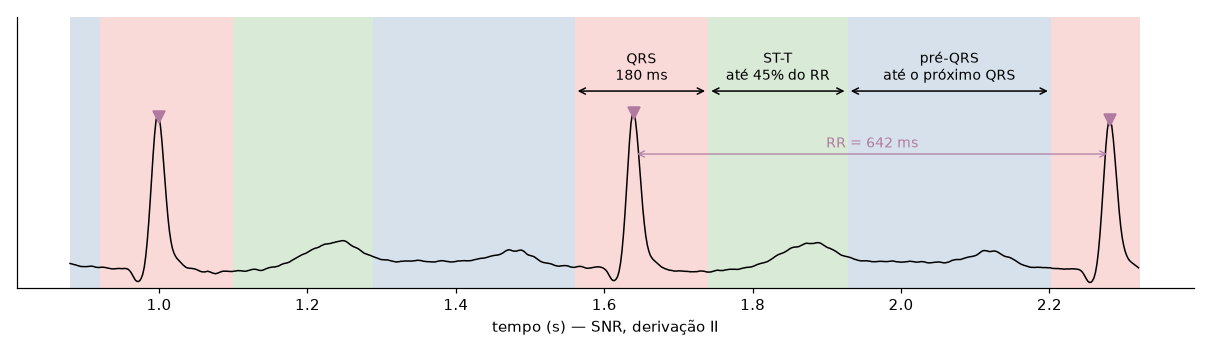
\includegraphics[width=0.8\textwidth]{figs/batimento.png}
\caption{Trecho de cerca de 1,5 s da derivação II de um ECG normal, com três picos R (triângulos) e as regiões de cada batimento: QRS (vermelho), ST-T (verde) e pré-QRS (azul). As mesmas regiões são aplicadas às 12 derivações.}
\label{fig:regioes}
\end{figure}

\subsection{O que cada métrica pergunta}
\begin{table}[H]
\centering
\small
\begin{tabularx}{\textwidth}{lXX}
\toprule
\textbf{Métrica} & \textbf{Pergunta} & \textbf{Como é calculada (versão atual)} \\
\midrule
Consistency & ECGs da mesma classe recebem a \textbf{mesma explicação}? & A explicação de cada mapa é o par das 2 regiões mais importantes, com o sinal; mede-se a fração dos outros mapas com o mesmo par que explicam a mesma classe. \\
\addlinespace
Faithfulness Correlation & A importância de um \textbf{grupo de regiões} corresponde ao efeito de retirá-lo do modelo? & 50 grupos sorteados de 9 regiões por ECG; correlação entre a soma das importâncias e a queda do \textit{logit}. \\
\addlinespace
Faithfulness Estimate & A importância de \textbf{cada região} corresponde ao efeito de retirá-la? & Cada uma das 36 regiões é retirada isoladamente; correlação entre a importância e a queda do \textit{logit}. \\
\bottomrule
\end{tabularx}
\end{table}
A Consistency olha a \textbf{estabilidade entre ECGs}; as duas Faithfulness olham a \textbf{fidelidade dentro de cada ECG}, com grupos (Correlation) ou uma região por vez (Estimate). Nas duas últimas, “retirar” é trocar a região pela baseline (zero ou média do treino, que deram resultados praticamente iguais).

\subsection{Faithfulness Estimate: reimplementada (novidade deste relatório)}
\textbf{O problema.} A configuração usada no Quantus trocava grupos de 500 pontos, em ordem de atribuição, pelo valor mínimo do próprio ECG. Num diagnóstico com 18 ECGs, retirar grupos de atribuição \textbf{negativa} derrubava o \textit{logit} quase tanto quanto retirar os de atribuição positiva (queda média de 3,06 contra 3,30). A métrica media o dano causado ao sinal, e não a retirada de informação.

\textbf{A versão atual.} Segue o artigo (Alvarez-Melis e Jaakkola, 2018): cada uma das 36 regiões é retirada isoladamente, e o valor do ECG é a correlação de Pearson entre a importância da região e a queda do \textit{logit}. Nos 622 mapas, retirar uma região de importância positiva baixa o \textit{logit} em 0,32, em média, e retirar uma de importância negativa o \textbf{aumenta} em 0,34, como se espera de uma explicação fiel. A implementação reaproveita o código da Faithfulness Correlation e foi conferida num caso sintético com resultado conhecido.

\subsection{Consistency, Faithfulness Correlation e Sufficiency}
Sem mudanças desde o último relatório. A Consistency e a Faithfulness Correlation foram reimplementadas porque, no Quantus, davam a mesma explicação para todos os ECGs (Consistency) ou criavam picos artificiais sem relação com as atribuições (Faithfulness Correlation). A Sufficiency foi retirada porque o próprio artigo não a define para métodos como o SHAP. Cada métrica tem um fichamento do artigo original com a comparação artigo × Quantus × versão atual.

\subsection{Complexidade: analisada}
O artigo da Faithfulness Correlation (Bhatt et al., 2020) propõe um terceiro critério, a \textbf{baixa complexidade}: uma explicação concentrada em poucos atributos é mais fácil de entender. A medida é a entropia das importâncias normalizadas. A versão do Quantus, ponto a ponto, não serve ao ECG: num diagnóstico com os 622 mapas, ela ordenou os mapas quase só pela duração do exame (correlação de postos de 0,88). Calculada por regiões, ela distingue os mapas (em média, as explicações usam o equivalente a 24 das 36 regiões) e não exige chamar o modelo. Propõe-se incluí-la como métrica \textbf{complementar}, lida ao lado da fidelidade. Como é de outra categoria do Quantus (nem fidelidade nem robustez), a inclusão amplia o escopo e ainda não foi feita. A análise completa está em \texttt{fichamentos/bhatt-2020-faithfulness-correlation/analise-complexidade.pdf}.

\section{Resultados (modelo B)}

\begin{table}[H]
\centering
\small
\caption{F1 e as três métricas por classe. Entre parênteses, a posição da classe em cada medida (1º = maior valor). Na Consistency, o valor esperado ao acaso aparece ao lado.}
\label{tab:res}
\begin{tabular}{lr rr rr rr rr}
\toprule
\textbf{Classe} & \textbf{Mapas} & \multicolumn{2}{c}{\textbf{F1}} & \multicolumn{2}{c}{\textbf{Consistency (acaso)}} & \multicolumn{2}{c}{\textbf{Faith.\ Corr.}} & \multicolumn{2}{c}{\textbf{Faith.\ Estimate}} \\
\midrule
BRD  & 172 & 0,927 & (2º) & 0,64 (0,23) & (1º) & 0,74 & (1º) & 0,78 & (1º) \\
IAVB &  61 & 0,884 & (3º) & 0,45 (0,08) & (3º) & 0,64 & (3º) & 0,57 & (5º) \\
AF   & 108 & 0,931 & (1º) & 0,42 (0,14) & (4º) & 0,54 & (6º) & 0,51 & (7º) \\
CVP  &  59 & 0,837 & (5º) & 0,26 (0,08) & (5º) & 0,61 & (4º) & 0,66 & (3º) \\
BRE  &  20 & 0,870 & (4º) & 0,25 (0,03) & (6º) & 0,65 & (2º) & 0,72 & (2º) \\
STD  &  65 & 0,778 & (7º) & 0,51 (0,09) & (2º) & 0,52 & (7º) & 0,51 & (9º) \\
SNR  &  78 & 0,796 & (6º) & 0,21 (0,10) & (7º) & 0,46 & (9º) & 0,51 & (8º) \\
CAP  &  45 & 0,750 & (8º) & 0,14 (0,06) & (8º) & 0,52 & (8º) & 0,55 & (6º) \\
STE  &  14 & 0,596 & (9º) & 0,03 (0,02) & (9º) & 0,60 & (5º) & 0,57 & (4º) \\
\midrule
\textbf{Global} & 622 & \textbf{0,819} & & \textbf{0,42 (0,13)} & & \textbf{0,61} & & \textbf{0,62} & \\
\bottomrule
\end{tabular}
\end{table}
Na Faithfulness Estimate, AF, SNR e STD diferem em menos de 0,01 e, na prática, empatam.

\begin{figure}[H]
\centering
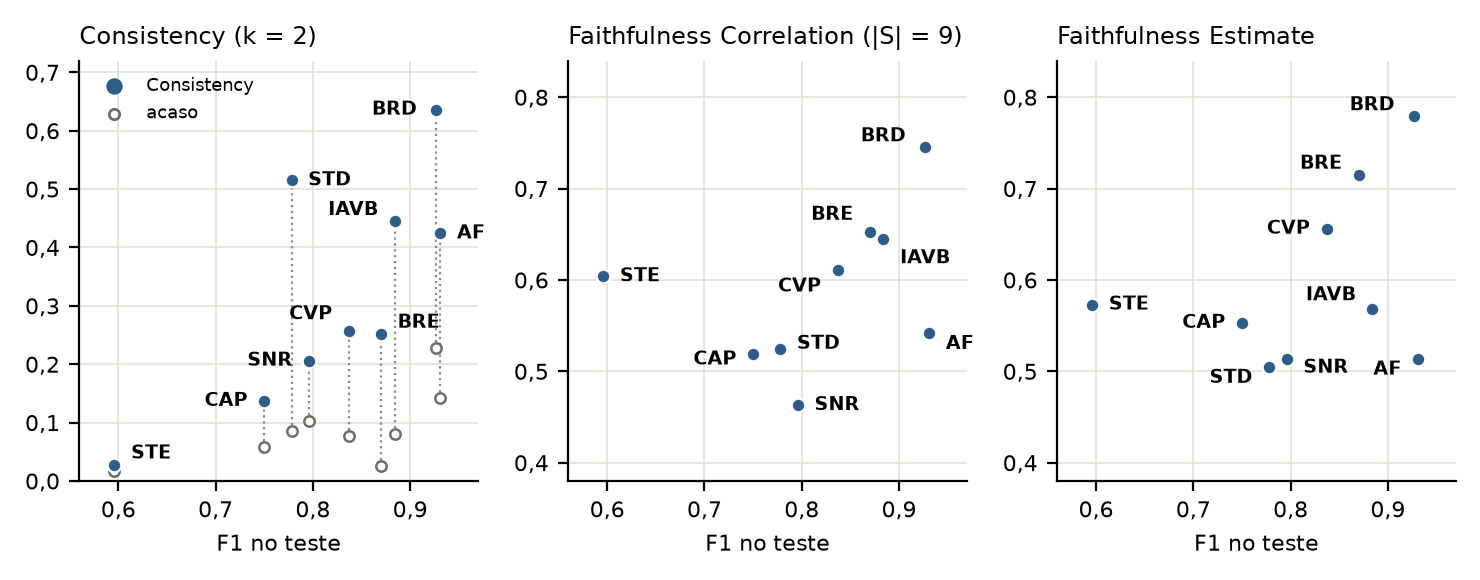
\includegraphics[width=\textwidth]{figs/f1_vs_metricas.png}
\caption{F1 por classe contra a Consistency (esquerda; círculos vazios: valor esperado ao acaso), a Faithfulness Correlation com grupos de 9 regiões (centro) e a Faithfulness Estimate (direita).}
\label{fig:disp}
\end{figure}

\section{O que as três métricas mostram em conjunto}

As comparações com o F1 são \textbf{descritivas} (ordenação das classes), sem coeficientes de correlação: as nove classes não são observações independentes (registros multirrótulo, mesmo modelo e mesmo conjunto de teste) nem uma amostra de uma população maior de classes.

\subsection{As explicações refletem o modelo, de forma moderada}
As três métricas apontam na mesma direção no nível global. A Consistency (0,42) é cerca de três vezes o esperado ao acaso (0,13): o SHAP tende a dar a mesma razão para ECGs da mesma classe. As duas Faithfulness ficam em torno de 0,6 e são positivas em todas as classes: as regiões que o SHAP aponta como importantes são, em geral, as que mais mudam a saída do modelo quando retiradas, e o sinal da importância indica a direção do efeito na maioria dos casos (68\%). Os valores são moderados, e não perfeitos: as explicações são informativas, mas não um retrato exato do modelo.

\subsection{Há duas dimensões de qualidade, e não três}
As duas Faithfulness concordam entre si: o valor global é quase o mesmo (0,61 e 0,62), e as classes ficam em ordem parecida (BRD e BRE no topo; SNR, STD, AF e CAP embaixo). Como uma retira grupos e a outra uma região por vez, a concordância mostra que a fidelidade medida não depende do tamanho do que se retira. Elas funcionam como \textbf{duas medidas da mesma dimensão}, a fidelidade. A Consistency é \textbf{outra dimensão}: várias classes têm posição muito diferente nas duas (STD é 2º na Consistency e 7º–9º na fidelidade; BRE é 6º na Consistency e 2º na fidelidade). Uma explicação pode ser fiel ao modelo em cada ECG sem se repetir entre ECGs, e vice-versa.

\subsection{Perfis das classes}
Cruzando as duas dimensões, as classes se dividem em quatro perfis:
\begin{table}[H]
\centering
\small
\begin{tabularx}{\textwidth}{lllX}
\toprule
\textbf{Perfil} & \textbf{Classes} & \textbf{F1} & \textbf{Leitura} \\
\midrule
Consistente e fiel & BRD, IAVB & 2º, 3º & O SHAP repete a mesma razão e ela corresponde ao efeito no modelo. \\
\addlinespace
Fiel, pouco consistente & BRE, CVP, STE & 4º, 5º, 9º & Cada explicação reflete o modelo, mas as regiões principais variam entre ECGs. \\
\addlinespace
Consistente, pouco fiel & STD, AF & 7º, 1º & A explicação se repete, mas a importância de cada região acompanha pior o efeito no modelo. \\
\addlinespace
Baixo nos dois & SNR, CAP & 6º, 8º & Explicações pouco repetidas e menos fiéis. \\
\bottomrule
\end{tabularx}
\end{table}

Alguns casos ajudam a entender o que está por trás desses perfis (dados da Faithfulness Estimate, que registra o efeito de cada região):
\begin{itemize}
    \item \textbf{BRD é o caso ideal.} A região mais importante é o QRS de V1 em 87\% dos mapas, que é o critério clínico do bloqueio de ramo direito; retirar regiões QRS é o que mais derruba a saída (0,58 em média); e a classe tem F1 alto. O modelo usa o critério esperado, e o SHAP o mostra de forma fiel e repetida.
    \item \textbf{IAVB também é coerente.} O bloqueio AV de 1º grau é um intervalo PR longo, que fica na região pré-QRS. O SHAP coloca 59\% da importância nessa região, e é ela que mais derruba a saída quando retirada.
    \item \textbf{AF: F1 mais alto, fidelidade baixa.} A fibrilação atrial é definida pelo \textbf{ritmo} (intervalos irregulares entre batimentos), e não pela forma de uma região. Retirar uma região não muda o momento dos batimentos, e de fato, para AF, retirar qualquer tipo de região quase não muda a saída em média (+0,07, +0,01 e $-$0,03, contra 0,58 do QRS no BRD). A fidelidade mais baixa de AF pode, portanto, refletir uma limitação das próprias regiões como unidade de medida para classes de ritmo, e não necessariamente uma explicação ruim.
    \item \textbf{STD: consistente, mas pouco fiel região a região.} O SHAP aponta repetidamente o segmento ST (aVR em 37\% dos mapas), e o tipo de região está certo (é a ST-T que mais derruba a saída). Mas a importância de cada derivação acompanha pior o efeito: STD tem a menor taxa de acerto do sinal (61\%). Uma hipótese é a redundância: o infradesnivelamento aparece em várias derivações, e retirar uma de cada vez tem efeito pequeno, porque as outras compensam.
    \item \textbf{STE: o pior F1 e nenhum padrão comum.} A Consistency é praticamente a do acaso (0,03 contra 0,02), mas a fidelidade é intermediária: cada explicação reflete o modelo, só que não há uma razão comum entre os ECGs. Além disso, tanto o SHAP quanto o efeito no modelo apontam para a região pré-QRS, e não para o segmento ST, onde o supradesnivelamento aparece. Isso sugere que o modelo não aprendeu um critério estável e clinicamente esperado para STE, o que é coerente com o F1 baixo (com a ressalva de que são só 14 mapas).
\end{itemize}

\subsection{O que isso diz sobre a pergunta do TCC}
A pergunta do TCC é se a qualidade das explicações acompanha o desempenho (F1) por classe. Até agora, a resposta é \textbf{“em parte”}:
\begin{enumerate}
    \item \textbf{Nas pontas há coincidência.} BRD está entre as melhores em F1 e é a melhor nas três métricas; STE e CAP, as duas de menor F1, têm as menores Consistency.
    \item \textbf{A Consistency acompanha o F1 melhor que a fidelidade.} Fora STD e AF, as posições na Consistency ficam próximas das posições no F1. Uma leitura possível: quando o modelo classifica bem uma classe, ele tende a usar uma razão estável, e o SHAP a repete entre ECGs.
    \item \textbf{A fidelidade parece depender mais do tipo de classe que do F1.} As classes definidas pela forma do QRS (BRD, BRE, CVP) têm as explicações mais fiéis; as definidas pelo ritmo ou pelo batimento como um todo (AF, SNR, CAP) têm as menos fiéis, mesmo com F1 alto no caso de AF.
    \item \textbf{Fidelidade não é correção clínica.} Uma explicação pode ser fiel ao modelo e apontar uma região inesperada (STE). As métricas avaliam se o SHAP descreve bem o modelo, e não se o modelo usa o critério clínico certo.
\end{enumerate}

\textbf{Limitações:} um único modelo e uma única divisão dos dados; apenas as predições corretas foram explicadas; classes pequenas (STE com 14 mapas, BRE com 20) têm valores menos estáveis; as regiões do batimento favorecem classes definidas por forma local e podem subestimar a fidelidade em classes de ritmo; as leituras por classe acima são hipóteses compatíveis com os dados, e não conclusões testadas.

\section{Revisão das demais métricas}

As métricas restantes seguem o mesmo procedimento: (1) leitura do artigo original; (2) comparação da implementação e da configuração do Quantus com a definição; (3) diagnóstico com dados; (4) se necessário, reimplementação adaptada ao ECG; (5) fichamento documentando as decisões.

\begin{table}[H]
\centering
\small
\caption{Situação das métricas.}
\begin{tabularx}{\textwidth}{lXl}
\toprule
\textbf{Métrica} & \textbf{Artigo de referência} & \textbf{Situação} \\
\midrule
\multicolumn{3}{l}{\textit{Fidelidade}} \\
Consistency & Dasgupta, Frost e Moshkovitz (2022) & Reimplementada e calculada \\
Faithfulness Correlation & Bhatt, Weller e Moura (2020) & Reimplementada e calculada \\
Faithfulness Estimate & Alvarez-Melis e Jaakkola (2018) & Reimplementada e calculada \\
Sufficiency & Dasgupta, Frost e Moshkovitz (2022) & Retirada \\
Sensitivity-N & Ancona et al. (2018) & Próxima a revisar (artigo já baixado) \\
Selectivity & Montavon, Samek e Müller (2018) & A revisar; estourava a memória (RAM) \\
Infidelity & Yeh et al. (2019) & A revisar; a mais cara de calcular \\
\midrule
\multicolumn{3}{l}{\textit{Complexidade}} \\
Complexity & Bhatt, Weller e Moura (2020) & Analisada; inclusão proposta (por regiões) \\
\midrule
\multicolumn{3}{l}{\textit{Robustez}} \\
Local Lipschitz Estimate & Alvarez-Melis e Jaakkola (2018) & A revisar; estourava a memória da GPU \\
Max- e Avg-Sensitivity & Yeh et al. (2019) & A revisar; estouravam a memória da GPU \\
Continuity & Montavon, Samek e Müller (2018) & A revisar; estourava a memória da GPU \\
RIS e ROS & Agarwal et al. (2022) & A revisar; estouravam a memória da GPU \\
\bottomrule
\end{tabularx}
\end{table}

\section{Próximos passos}
\begin{itemize}
    \item Revisar a Sensitivity-N, cujo artigo já foi baixado, seguida das demais métricas de fidelidade.
    \item Definir a inclusão da complexidade por regiões como métrica complementar.
    \item Revisar as métricas de robustez, resolvendo também os problemas de memória da GPU.
    \item Acrescentar cada métrica revisada à análise conjunta, verificando se os perfis das classes descritos na seção~5 se mantêm.
\end{itemize}

\end{document}
